\documentclass[fontsize=12pt,paper=a4,DIV12,cleardoublepage=empty, 
liststotoc,idxtotoc,bibtotoc]{article}
\usepackage[ngerman]{babel}
\usepackage[utf8]{inputenc}
\usepackage[pdftex]{graphicx}
\usepackage{amsmath}
\usepackage{longtable}
\usepackage{stmaryrd}
\usepackage{colortbl}
\usepackage{eurosym}
\usepackage{amssymb}
\usepackage{amsthm}
\usepackage{nicefrac}
\usepackage{lscape}
\usepackage{pdfpages} 
%Seitenlayout
\renewcommand{\thesection}{\Roman{section}}
\renewcommand{\thesubsection}{\Roman{section}.\arabic{subsection}}
\usepackage[left=25mm, right=25mm, bottom=30mm]{geometry}
\usepackage[doublespacing]{setspace}
\usepackage[colorlinks=true, linkcolor=black, citecolor=black, urlcolor=blue]{hyperref} 
\usepackage[figure]{hypcap}
%Textstruktur
\usepackage{float}
\usepackage{wrapfig}
\usepackage{tabularx}
%Textaussehen
\usepackage{framed}
%Verzeichnisse
\usepackage{csquotes}
\usepackage[backend=biber, bibstyle=authoryear-ibid, uniquelist=false, maxbibnames=9, maxcitenames=3, citestyle=authoryear-icomp, isbn=true, url=true, block=space, pagetracker=page,   giveninits=false, dateabbrev=false, dashed=false ]{biblatex}
\addbibresource{MA_literatur.bib}
\DefineBibliographyStrings{ngerman}{ 
	andothers = {{et\,al\adddot}},             
} 
\usepackage{etoolbox}
\apptocmd{\UrlBreaks}{\do\f\do\m}{}{}
\setcounter{biburllcpenalty}{9000}% Kleinbuchstaben
\setcounter{biburlucpenalty}{9000}% Großbuchsta
\expandafter\def\expandafter\quote\expandafter{\quote\small\singlespacing}

\setcounter{section}{0}
\setcounter{subsection}{0}

\newcommand*{\meincite}[1]{\citeauthor{#1} (\citeyear{#1})}

\newcommand{\KK}{\mathbb{•}{K}}
\newcommand{\CC}{\mathbb{C}}
\newcommand{\RR}{\mathbb{R}}
\newcommand{\QQ}{\mathbb{Q}}
\newcommand{\ZZ}{\mathbb{Z}}
\newcommand{\NN}{\mathbb{N}}
\newcommand{\PPO}{\mathcal{P}(\Omega)}

\theoremstyle{plain}
\newtheorem{satz}{Satz}[subsection]
\newtheorem{lem}[satz]{Lemma}
\newtheorem{theo}[satz]{Theorem}
\newtheorem{kor}[satz]{Korollar}
\newtheorem{defi}{Definition}
\theoremstyle{definition}
\newtheorem{bei}[satz]{Beispiel}
\newtheorem{bem}[satz]{Bemerkung}

\graphicspath{ {./images/} }

\begin{document}
	\definecolor{gold}{rgb}{0.9,0.9,0}
	\begin{titlepage}
		\vspace*{-3cm}
		\noindent
		\hspace*{1cm}
			\begin{center}
				\centering
				{\LARGE Gesamtschule Scharnhorst}
			\end{center}
		\begin{center}
		\Large{Fundamentalsatz der Analysis}\\[0.5cm]
		\normalsize{geschrieben von}\\[0.25cm]	
		\large{Benno Schörmann}\\[0.5cm]
		\end{center}
	\begin{flushleft}
	\hyperref[subsec:thema1]{\textbf{\large Thema der Facharbeit:}}  \\
	\end{flushleft}
	Eine vollständige Definition und ein vollständiger Beweis des Fundamentalsatzes der Analysis
	\quad \\[1.5cm]
	\noindent 
	\renewcommand{\arraystretch}{1.4}
	\end{titlepage}
	\newpage
	\thispagestyle{empty}
	\tableofcontents
	\newpage
	%\listoffigures
	%\thispagestyle{empty}
	%\newpage	
	\section{Einleitung}
	(Die Einteilung steht übrigens noch absolut nicht fest, habe sie gestern abend im Halbschlaf angefertigt) \\\\
	In dieser Facharbeit werde ich über Den Fundamentalsatz der Analysis und die dazugehörigen Nebenpunkte schreiben.
	
	
	
	\section{Geschichtliche Zusammenfassung}
	%Newton/Gauss Fight\\
	%Jahreszeiten, Semi guter Beweis am Anfang?\\
	%\footnote{Omar A. Hernandez Rodriguez (University of Puerto Rico) and Jorge M. Lopez Fernandez (University of Puerto Rico), "Teaching the Fundamental Theorem of Calculus: A Historical Reflection - Integration from Cavalieri to Darboux," Convergence (Januar 2012)}
	Die Geschichte des Hauptsatzes der Differential- und Integralrechnung beginnt im 17. Jahrhundert mit Gottfried Leibnitz und Isaac Newton. Leibnitz sah das Integral als eine unendlich große Menge an Flächen die unendlich klein sind. Damit zeigte er den wichtigen Zusammenhang zwischen Integration und Fläche. Isaac Newton nutzte die Geometrie, um den Unterschied zwischen Distanz, Geschwindigkeit und Beschleunigung zu beschreiben. Das ist der Schlüssel, um das Verhältnis zwischen Integral und Ableitung zu verstehen. Krümmung ist die Ableitung von Steigung und Steigung ist die Ableitung von Strecke/Distanz. Distanz ist hingegen das Integral von Steigung und Steigung ist das Integral von Krümmung. 1823 hat Cauchy das Integral per Limes definiert. In dem 19. Jahrhundert hat Siméon Denis Poisson das Integral als  \footnote{Bressoud, D. (2011). “Historical reflections on teaching the fundamental theorem of integral calculus.” The American Mathematical Monthly, 118(2), 99-115}
	%\footnote{https://simple.wikipedia.org/wiki/Fundamental_theorem_of_calculus}
	
	

	\section{Alle wichtigen Begriffe erklärt}
	Anschauliche Beispiele? (Scipy Einbindung?)
	
	
	\subsection{Was ist Differentialrechnung?}
	-eines der am einfachsten zu begreifenden Themen der Analysis ermöglicht dieser Teil der Analysis das finden von Extrema und das generelle Beschreiben von Funktionsverläufen.
	
	
	\subsubsection{Wie wird eine Funktion abgeleitet?}
		Text
	
	
	\subsection{Was ist Integralrechnung?}
		Text


	\subsubsection{Wie wird eine Funktion integriert?}
		Text
		
	
	\subsection{Was ist eine stetige Funktion?}
		Text	
	
	
	\section{Mittelwertsatz der Integralrechnung}
	\begin{satz}" "\\
		Gegeben ist die in $\RR$ definierte Funktion auf dem Intervall $[a, b]$ liegende Funktion $f$ und $g$. $g$ ist außerdem integrierbar und ohne Vorzeichenwechsel, also $g \geq 0$ \textbf{oder} $g \leq 0$. Dann existiert mindestens ein $\xi$, sodass
		\begin{equation*}
			\int_{a}^{b}f(t)g(t)dt=f(\xi)\int_{a}^{b}g(t)dt			
		\end{equation*}
		Die obrige Aussage wird auch als erweiteter Mittelwertsatz bezeichnet. Wenn allerdings $g=1$ ist, kommt es zu einem spezialgelagerten Sonderfall\\
		%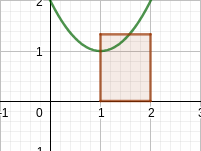
\includegraphics[scale=0.3]{Mittelwertsatz xTo2.png}
		\begin{equation*}
			\int_{a}^{b}f(t)dt=f(\xi)(b-a)
		\end{equation*}
		Wenn man die rechte seite der Gleichung bertachtet, fällt auf, dass dort der eines Rechtecks gebildet wird. Dieses Rechteck hat die gleiche Fläche wie das Integral zwischen $a$ und $b$.		
		
	\end{satz}
	
	\begin{proof}" "\\
		Gegeben ist die in $\RR$ definierte Funktion $g$, wobei $g(x)\geq0$ und auf dem Intervall $[a, b]$ liegt.\\
		$f$ nimmt zwischen $a$ und $b$ ein Minimum $k$ und ein Maximum $K$ an. Somit ist $k \leq f(x) \leq K$ und bei $g\geq0$ ist $kg(x)\leq f(x)g(x)\leq Kg(x)$. Daraus erschließt sich
		\begin{equation*}
			k \int_{a}^{b}g(x)dx \leq \int_{a}^{b}f(x)g(x)dx\leq K\int_{a}^{b}g(x)dx
		\end{equation*}
	\end{proof}
	
	
	\section{Hauptsatz der Differential- und Integralrechnung}
	
	Der Hauptsatz der Differential- und Integralrechnung ist in zwei Hauptsätze und einen Nebensatz aufgeteilt. Der erste Satz stellt den Zusammenhang zwischen Integral und Differential dar.

	\subsection{Erster Teil}
	\begin{satz}" "\\
		Gegeben ist die in $\RR$ definierte Funktion $f$ in einem geschlossenen Intervall $[a, b]$. Sei $F$ definiert für alle $x$ im Intervall $[a, b]$ durch \\
			\begin{equation*}
				F(x)=\int_{a}^{x}f(t) dt
			\end{equation*}
		Dann ist $F$ gleichmäßig stetig auf dem Intervall $[a, b]$ und differenzierbar auf dem offenen Intervall $(a, b)$, und 
			\begin{equation*}
				F'(x)=f(x)
			\end{equation*}
		Für alle $x$ in $(a, b)$, sodass $F$ eine Stammfunktion von $f$ ist.\\\\
	
	\end{satz}
	
	
	\begin{proof}" "\\
		Für ein gegebenes $f(t)$ sei die Funktion $F(x)$ definiert als
		\begin{equation*}
			F(x)=\int_{a}^{x}f(t)dt
		\end{equation*}
		Für jegliche 2 Zahlen $x_1$ und $\Delta x$ im Intervall $[a, b]$ ergibt sich
		\begin{equation*}
			F(x_1)=\int_{a}^{x_1}f(f)dt
		\end{equation*}
		und
		\begin{equation*}
			F(x_1+\Delta x)=\int_{a}^{x_1+\Delta x}f(t)dt
		\end{equation*}
		Wenn diese beiden Gleichungen nun subtrahiert werden, dann ergibt sich
		\begin{equation}
			F(x_1+\Delta x)-F(x_1)=\int_{a}^{x_1+\Delta x}f(t)dt-\int_{a}^{x_1}f(t)dt
		\end{equation}
		Die Summe beider Flächen ist
		\begin{equation*}
			\int_{a}^{x_1}f(t)dt + \int_{x_1}^{x_1+\Delta x}f(t)dt = \int_{a}^{x_1+\Delta x}f(t)dt
		\end{equation*}
		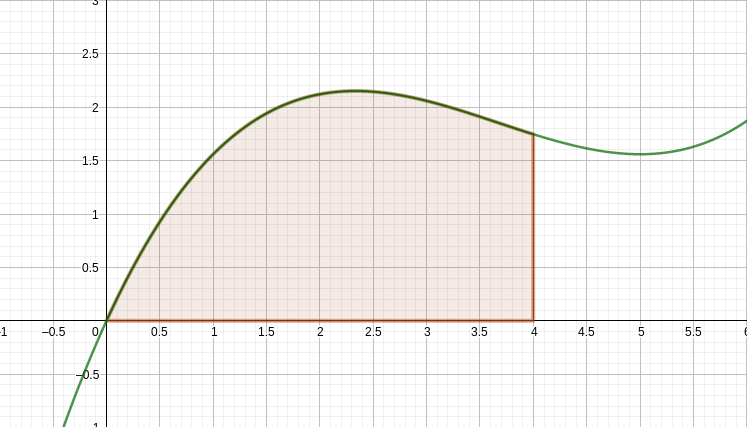
\includegraphics[scale=0.2]{Integral 0-4.png} $+$
		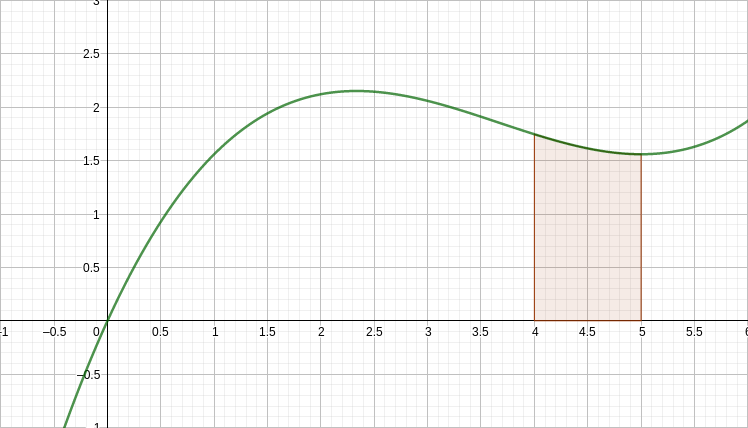
\includegraphics[scale=0.2]{Integral 4-5.png} $=$
		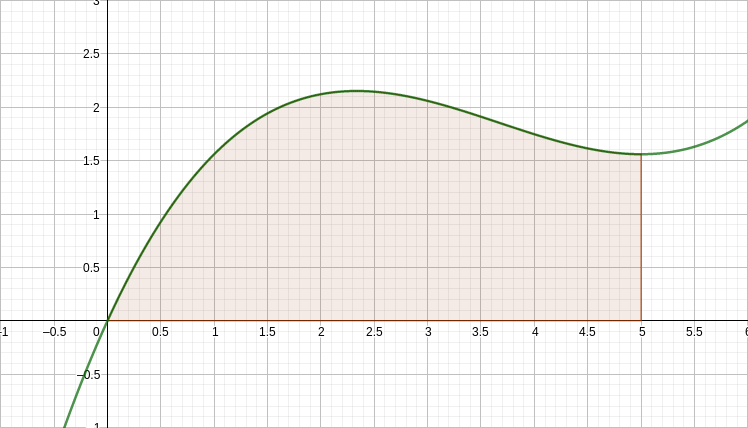
\includegraphics[scale=0.2]{Integral 0-5.png} \\
		Wenn man, wie in dem oben gezeigten Fall, die Flächen zweier Integrale von z.B. 0 bis 4 und 4 bis 5 addiert, dann ergibt das die Fläche des Integrals von 0 bis 5. Generell ausgedrückt ist das also
		\begin{equation*}
			\int_{a}^{b}f(t)dt + \int_{b}^{c}f(t)dt = \int_{a}^{c}f(t)dt
		\end{equation*}
		, wobei $a\leq b\leq c$.\\
		Die Umformung dieser Gleichungen gibt
		\begin{equation*}
			\int_{a}^{x_1+\Delta x}f(t)dt-\int_{a}^{x_1}f(t)dt=\int_{x_1}^{x_1+\Delta x}f(t)dt
		\end{equation*}
		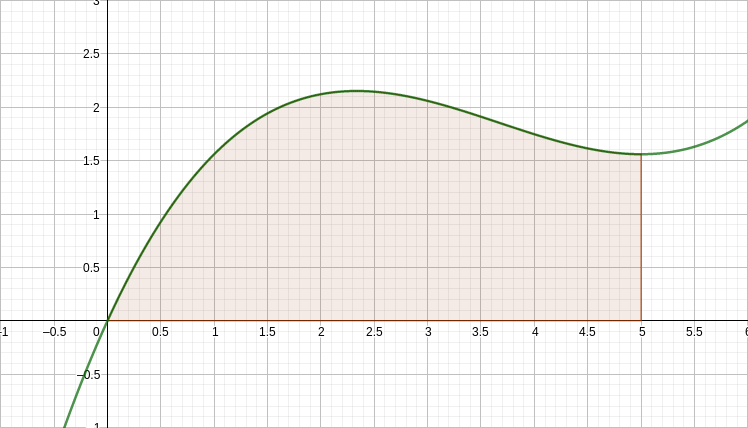
\includegraphics[scale=0.2]{Integral 0-5.png} $-$
		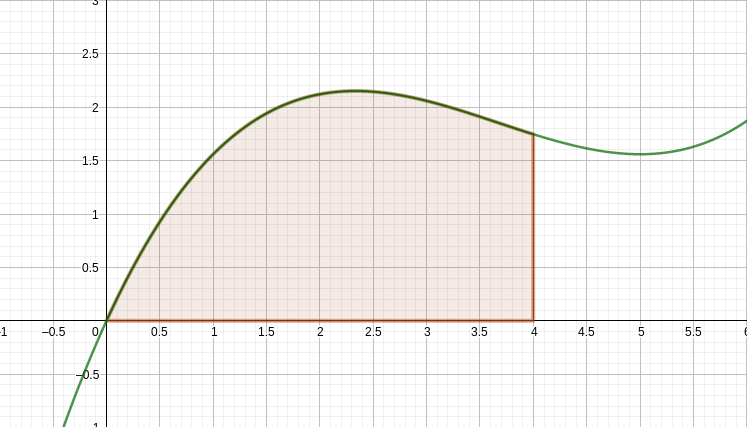
\includegraphics[scale=0.2]{Integral 0-4.png} $=$
		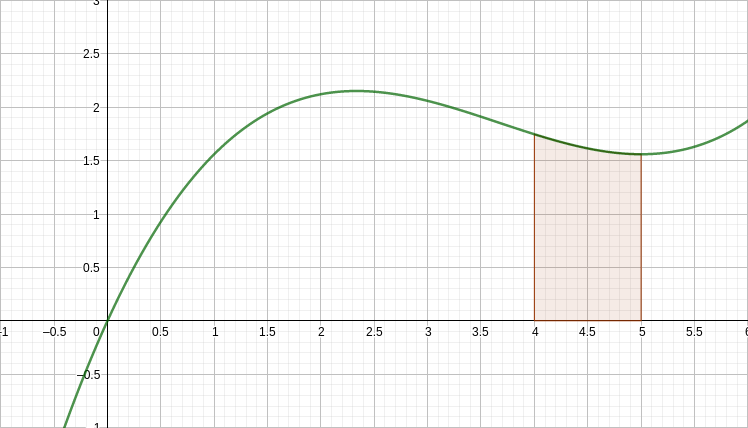
\includegraphics[scale=0.2]{Integral 4-5.png} \\
Wenn man, wie in dem oben gezeigten Fall, die Flächen zweier Integrale von z.B. 0 bis 5 und 0 bis 4 miteinander subtrahiert, dann ergibt das die Fläche des Integrals von 4 bis 5. Generell ausgedrückt ist das also
		\begin{equation*}
			\int_{a}^{c}f(t)dt - \int_{a}^{b}f(t)dt = \int_{b}^{c}f(t)dt
		\end{equation*}
		, wobei $a\leq b\leq c$.\\
		Nun wird die Gleichung (1) eingesetzt.
		\begin{equation}
			F(x_1+\Delta x)-F(x_1)=\int_{x_1}^{x_1+\Delta x}f(t)dt
		\end{equation}
		Laut dem Mittelwertsatz der Integralrechung gibt es eine Zahl c in $[x_1, x_1+\Delta x]$, sodass
		\begin{equation}
			\int_{x_1}^{x_1+\Delta x}f(t)dt=f(c)*\Delta x
		\end{equation}
		Nun wird die Gleichung (2) und (3) zusammengefügt und durch $\Delta x$ dividiert
		\begin{equation*}
			F(x_1+\Delta x)-F(x_1)=f(c)*\Delta x \;\;\;\;|\div \Delta x
		\end{equation*}
		\begin{equation*}
			\frac{F(x_1+\Delta x)-F(x_1)}{\Delta x}=f(c)
		\end{equation*}
		Auffallend ist, dass die linke Seite zu einem Differenzeinquotienten umgeformt wurde. Wird nun $\lim \limits_{\Delta x \to 0}$ angewandt, dann
		\begin{equation*}
			\lim \limits_{\Delta x \to 0} \frac{F(x_1+\Delta x)-F(x_1)}{\Delta x}=\lim \limits_{\Delta x \to 0}f(c)
		\end{equation*}
		Und somit
		\begin{equation}
			F'(x_1)=\lim \limits_{\Delta x \to 0}f(c)
		\end{equation}
		Nun fehlt nur noch $f(c)$.\\ Da $x_1 \leq c \leq x_1+\Delta x$ ist und $\Delta x$ gegen $0$ läuft wird sich $c\to$ $x_1$ nähern bis bei $\Delta x=0$ auch $c = x_1$ ist, beziehungsweise $x_1 \leq c \leq x_1 + 0$ oder $x_1 = c = x_1$ ist.\\Zusammenfassend ist also
		\begin{equation}
			\lim \limits_{\Delta x \to 0} f(c) = f(x_1)
		\end{equation}
		Und somit, wenn man (4) und (5) zusammenfügt
		\begin{equation*}
			F'(x_1)=f(x_1)
		\end{equation*}
		Eine andere Schreibweise wäre
		\begin{equation*}
			\frac{d}{dx}\int_{a}^{x}f(t)dt=f(x)
		\end{equation*}
		Damit ist der erste Satz der Differential- und Integralrechnung bewiesen.
	\end{proof}
	\newpage
	
	
	\subsection{Korollar}
	\begin{satz}" "\\
		Gegeben ist die in $\RR$ definierte, auf dem Intervall $[a, b]$ stetige Funktion $f$  und $F$ eine Stammfunktion von $f$ im Intervall $[a, b]$, dann gilt
		\begin{equation*}
			\int_{a}^{b}f(t)dt=F(b)-F(a)
		\end{equation*}
		Das Korollar erfordert Stetigkeit auf dem ganzen Intervall.
	\end{satz}

	\begin{proof}" "\\
		Sei $F$ ein Stammfunktion von $f$ mit Stetigkeit auf dem Intervall $[a, b]$, dann sei
		\begin{equation*}
			G(x)=\int_{a}^{x}f(t)dt
		\end{equation*}
		Durch den ersten Beweis ist bewiesen, dass $G(x)$ eine Stammfunktion von f ist. Da $F'(x)-G'(x)=0$ ist der Mittelwertsatz der Integralrechnung impliziert, dass $F(x)-G(x)$ eine konstante Funktion ist, das heißt es gibt eine Zahl $c$, so dass $G(x)=F(x)+c$ für alle $x$ in $[a, b]$. Es gilt also
		\begin{equation*}
			F(a)+c=G(a)=\int_{a}^{a}f(t)dt=0
		\end{equation*}
		Das bedeutet, dass $c=-F(a)$. In anderen Worten, $G(x)=F(x)-F(a)$, und somit
		\begin{equation*}
			\int_{a}^{b}f(t)dt=G(b)=F(b)-F(a)
		\end{equation*}
		Somit ist das Korollar des Hauptsatzes der Differential- und Integralrechnung bewiesen.
	\end{proof}	
	\newpage
	
	
	\subsection{Zweiter Teil}
	
	\begin{satz}" "\\
	Dieser Teil wird manchmal Zweiter Teil des Hauptsatzes der Differential- und Integralrechnung oder das Newton-Leibniz-Axiom genannt.\\
	Gegeben ist die in $\RR$ definierte Funktion $f$ auf dem geschlossenen Intervall $[a, b]$, und $F$, eine Stammfunktion von $f$ auf dem Intervall $(a, b)$
	\begin{equation*}
		F'(x)=f(x)
	\end{equation*}
	Wenn $f$ auf dem Intervall $[a, b]$ Riemann-integrierbar ist, dann 
	\begin{equation*}
		\int_{a}^{b}f(x)dx=F(b)-F(a)
	\end{equation*}
	Der zweite Teil ist aussagekräftiger als das Korollar, da er nicht voraussetzt, dass $f$ eine stetige Funktion ist.\\
	Wenn eine Stammfunktion $F$ von $f$ existiert, dann gibt es unendlich viele unterschiedliche Stammfunktionen die erlangt werden, indem eine Konstante, oftmals $c$ genannt, an $F$ addiert wird. Außerdem existiert laut dem ersten Teil eine Stammfunktion $F$, sobald $f$ kontinuierlich ist, was durch das nicht Vorhandensein einer Stammfunktion von Funktionen, wie $e^{-x^2}$ widerlegt ist.
	
	\end{satz}	
	
	\begin{proof} " "\\
	Dies ist ein Grenzbeweis durch die Riemann-Summe. Sei $f$ Riemann-integrierbar auf dem Intervall $[a, b]$ und lasse $f$ eine Stammfunktion $F$ auf dem Intervall $[a,b]$ zu. $F(b)-F(a)$. Seien $x_0 \cdots x_n$, sodass
	\begin{equation*}
		a = x_0 < x_1 < x_2 < \cdots < x_{n-2} < x_{n-1} < x_n = b
	\end{equation*}
	Daraus lässt sich erschließen, dass
	\begin{equation*}
		F(b)-F(a)=F(x_n)-F(x_0)
	\end{equation*}
	Nun wird jedes $F(x_k)$ zusammen mit seinem negativen gegenpart addiert, sodass die daraus ergebende menge folgendes ergibt
	\begin{multline*}
	\begin{aligned}
		F(b)-F(a)=& F(x_n)+[-F(x_{n-1})+F(x_{n-1})]+[-F(x_{n-2})+F(x_{n-2})]+\cdots +\\ &[-F(x_2)+F(x_2)]+[-F(x_1)+F(x_1)]-F(x_0)\\
		=& [F(x_n)-F(x_{n-1})]+[F(x_{n-1})-F(x_{n-2})]+\cdots+[F(x_2)-F(x_1)]+[F(x_1)-F(x_0)]
	\end{aligned}
	\end{multline*}
	Die obere Menge kann folgendermaßen zusammengefasst werden
	\begin{equation}
		F(b)-F(a)=\sum_{k=1}^{n} [F(x_k)-F(x_{k-1})]
	\end{equation}
	Als nächstes wird der Mittelwertsatz der Integralrechnung benötigt. Kurz zusammengefasst:\\
	Sei $F$ stetig auf dem geschlossenen Intervall $[a, b]$ und differenzierbar auf dem offenen Intervall $(a, b)$, dann existiert ein $c$ im Intervall $(a, b)$, sodass 
	\begin{equation*}
		F'(c)=\frac{F(b)-F(a)}{b-a}
	\end{equation*}
	Daraus folgt
	\begin{equation*}
		F'(c)(b-a)=F(b)-F(a)
	\end{equation*}
	$F$ ist differenzierbar auf dem Intervall $[a, b]$ und somit auch differenzierbar auf dem Intervall $[x_{k-1}, x_k]$. Laut dem Mittelwertsatz der Integralrechnung ergibt sich somit
	\begin{equation}
		F(x_k)-F(x_{k-1})=F'(c_k)(x_k-x_{k-1})
	\end{equation}
	Nun wird das Ergebnis von (7) in die Gleichung von (6) eingesetzt
	\begin{equation*}
		F(b)-F(a)=\sum_{k=1}^{n} [F'(c_k)(x_k-x_{k-1})]
	\end{equation*}
	Vorausgesetzt wird, dass $F'(c_k)=f(c_k)$ ist. Außerdem kann einfachheitshalber $(x_k-x_{k-1})$ als $\Delta x$ des Teils $k$ geschrieben werden, also $\Delta x_k$
	\begin{equation}
		F(b)-F(a)=\sum_{k=1}^{n} [f(c_k)(\Delta x_k)]
	\end{equation}
	--add text--\\
	Nun wird Limes $\Delta x_k \to 0$ angewendet. Dies bewirkt, dass die Einteilungen, auch Partitionen genannt, gen 0 gehen und die Genauigkeit des Intervalls immer besser wird, da es immer weniger Überschuss oder Ungenauigkeiten gibt.
	\begin{equation*}
		\lim \limits_{\Delta x_k \to 0} F(b)-F(a)=\lim \limits_{\Delta x_k \to 0} \sum_{k=1}^{n} [f(c_k)(\Delta x_k)]
	\end{equation*}
	Da $F(b)-F(a)$ kein $\Delta x_k$ beinhaltet bleibt diese Seite der Gleichung unverändert bestehen und somit bleibt
	\begin{equation*}
		F(b)-F(a)=\lim \limits_{\Delta x_k \to 0} \sum_{k=1}^{n} [f(c_k)(\Delta x_k)]
	\end{equation*}
	Die rechte Seite der Gleichung definiert das Integral von $f$ von $a$ bis $b$. Somit ergibt sich
	\begin{equation*}
		F(b)-F(a)=\int_{a}^{b}f(x)dx
	\end{equation*}
	Somit ist der Zweite Teil des Hauptsatzes der Differential- und Integralrechnung bewiesen.
	\end{proof}
	
	
	
	\section{Auswirkungen auf die Mathematik}
	
	
	
	\printbibliography[title=Literaturverzeichnis]


\end{document}